\chapter{Amber at a Glance}
\label{ch:overview}

\begin{defbox}[In this chapter you will learn]
\begin{itemize}
 \item the three entity types Amber simulates and how they interact;
 \item the life cycle of a single node, told with real simulator output;
 \item the four design principles stated in the paper and how each is realised;
 \item the time scales involved, and a one-page walk-through of a single poll;
 \item a map of the rest of the book, so every later detail has a home.
\end{itemize}
\end{defbox}

\section{Three entity types}

The paper states that Amber ``models three entity types: nodes, base stations,
and the communication links between them.'' Let us fix what each one is.

\paragraph{Nodes.} Stationary, passive, battery-free devices. A node is
characterised by its \emph{position}, its \emph{antenna gain}, its
\emph{receiver sensitivity} (the weakest command it can notice) and a
\emph{power split ratio} that says how the received RF power is divided
between energy harvesting and backscatter reflection. Its behaviour is driven
by two voltage thresholds, $\Vhigh$ and $\Vlow$ (Chapter~\ref{ch:capacitor}).

\paragraph{Base stations.} Each base station has several \emph{sectors}. A
sector is described by its azimuth, beamwidth, height, antenna gain, transmit
power, receiver sensitivity and a 3GPP-compliant antenna pattern
(Chapter~\ref{ch:antennas}). The base station provides the \emph{carrier} (power
and backscatter illumination), sends \emph{commands} to nodes, and
\emph{receives} the reflected replies.

\paragraph{Links.} ``Communication links are computed bidirectionally:
downlink for wireless power transfer and carrier provision, uplink for
backscattered data.'' Because nodes and base stations do not move, both
directions are computed \emph{once, before the simulation starts}, and then
simply looked up.

\begin{figure}[t]
\centering
\begin{tikzpicture}[x=1cm,y=1cm]
 % --- base station ----------------------------------------------------
 \draw[rounded corners=3pt,draw=ablue,fill=lightblue] (0,-0.9) rectangle (4.1,5.1);
 \node[lab,anchor=south] at (2.05,5.1) {\textbf{Base station} (\code{BSBehavior})};
 \node[box,fill=white,draw=aorange,minimum width=3.4cm] (sch) at (2.05,4.15) {schedule or\\policy of frames};
 \node[box,fill=white,draw=aorange,minimum width=3.4cm] (rxw) at (2.05,2.55) {RX window: buffer,\\ collisions, SIC, ACKs};
 \node[box,fill=white,draw=aorange,minimum width=3.4cm] (cw)  at (2.05,0.75) {sectors + antennas\\carrier (always on)};
 \draw[->] (sch) -- node[lab,right]{commands} (rxw);
 % --- node -------------------------------------------------------------
 \draw[rounded corners=3pt,draw=agreen,fill=lightgreen] (8.1,-0.9) rectangle (15.3,5.6);
 \node[lab,anchor=south] at (11.7,5.6) {\textbf{Node} (\code{Controller} + \code{Capacitor} + \code{BackscatterModule})};
 \node[box,minimum width=1.5cm] (spl) at (9.3,2.35) {split\\$\eta:1{-}\eta$};
 \node[box,draw=agreen,minimum width=3.1cm] (har) at (12.8,4.5) {harvester\\$V_{\mathrm{src}}=\sqrt{P_h\Rs}$};
 \node[box,draw=agreen,minimum width=3.1cm] (cap) at (12.8,3.0) {capacitor $C$\\$V$ vs $\Vhigh,\Vlow$};
 \node[box,draw=agreen,minimum width=3.1cm] (ctl) at (12.8,1.5) {controller FSM\\listen/sense/proc/TX};
 \node[box,draw=agreen,minimum width=3.1cm] (bsm) at (12.8,0.0) {protocol \& backscatter\\(\code{send_id}, \code{send_data})};
 \draw[->] (har) -- (cap);
 \draw[->] (cap) -- node[lab,right]{$V$} (ctl);
 \draw[->] (ctl.west) .. controls +(-0.75,0) and +(-0.75,0) .. node[lab,left,pos=0.5]{$I_L$} (cap.west);
 \draw[<->] (ctl) -- node[lab,right]{ready?} (bsm);
 \draw[->] (spl.north) |- node[lab,above,pos=0.8]{harvest} (har.west);
 \draw[->] (spl.south) |- node[lab,below,pos=0.8]{reflect} (bsm.west);
 \node[ext] (sol) at (12.8,6.55) {external source\\(solar trace)};
 \draw[->] (sol) -- (har);
 % --- links -------------------------------------------------------------
 \draw[->,line width=1.1pt,ablue] (4.1,3.9) -- node[above,lab,align=center]{downlink: carrier tone\\+ data subcarrier} (spl.west |- 4.1,3.9) -- (9.3,3.9) -- (spl.north west);
 \draw[->,line width=1.1pt,aorange] (spl.south west) -- (9.3,0.7) -- node[below,lab,align=center]{uplink: backscatter\\(shifted subcarrier)} (4.1,0.7);
\end{tikzpicture}
\caption{Energy and information flow in Amber. The base station radiates a carrier; a node splits the received power between harvesting and reflection. Energy flows downward through the harvester into the capacitor; the controller turns capacitor voltage into duty-cycled activity and permits the protocol module to answer.}
\label{fig:overview}
\end{figure}

\section{The life of a node}
\label{sec:lifeofnode}

Figure~\ref{fig:sawtooth} shows the capacitor voltage of three nodes during a
20-second run of the shipped broadcast demo. This is \emph{real output} of
the simulator; reading it carefully teaches most of what follows.

\begin{figure}[t]
\centering
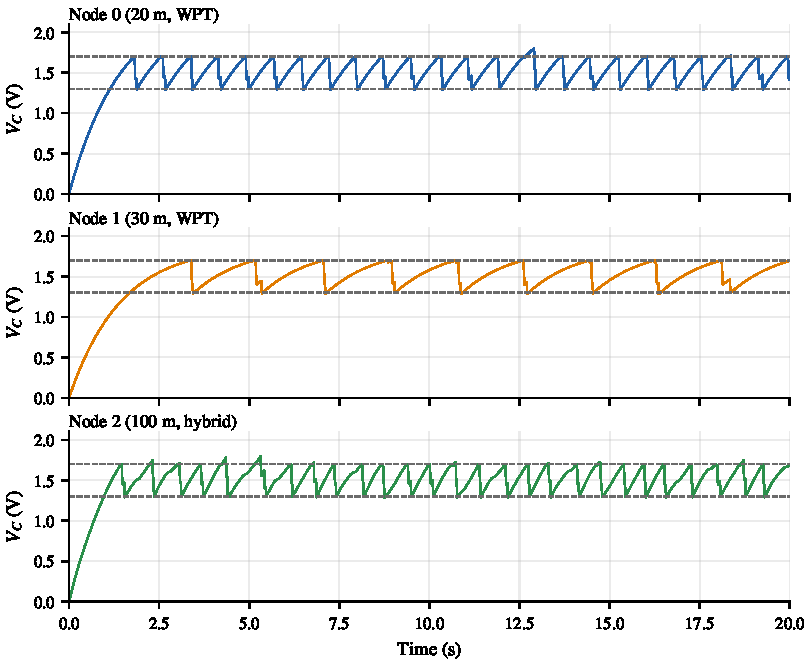
\includegraphics[width=0.92\linewidth]{fig_sawtooth}
\caption{Capacitor voltage of the three nodes of the broadcast demo (measured; random seed fixed for the figure). Node~0 and Node~1 harvest only from the base station's carrier at \SI{20}{m} and \SI{30}{m}. Node~2 is \SI{100}{m} away, too far to power itself from RF alone, and runs on its \emph{solar} trace instead. Dashed lines: $\Vhigh=\SI{1.7}{V}$ and $\Vlow=\SI{1.3}{V}$.}
\label{fig:sawtooth}
\end{figure}

\begin{enumerate}
 \item \textbf{Charging.} All capacitors start empty. Each rises along an RC
   curve towards the equivalent source voltage determined by the harvested
   power. The closer node reaches $\Vhigh=\SI{1.7}{V}$ sooner (about
   \SI{1.8}{s} for Node~0, about \SI{3.4}{s} for Node~1).
 \item \textbf{Activation.} Once $V\ge\Vhigh$ (and a random start-up delay of
   up to two seconds has elapsed), the node becomes \emph{active} and starts its
   duty cycle.
 \item \textbf{Duty-cycling.} Each time the node backscatters a packet it pays a
   large current for a few milliseconds---the sharp downward steps. Between
   packets it charges again---the slanted ramps.
 \item \textbf{Shut-down.} When the voltage falls to $\Vlow=\SI{1.3}{V}$ the node
   switches off and charges back up. The \emph{saw-tooth} is the signature of
   threshold-driven intermittent operation.
\end{enumerate}
The three traces differ in a way the radio alone would not predict. Node~2 is the farthest yet charges the \emph{fastest}, because the simulator
lets it draw on an external (solar) source; it also sends the most packets.
In the demo's 20-second run Node~0, Node~1 and Node~2 sent about 46, 18 and 58
packets respectively (counts vary slightly between runs). \textbf{Communication range is not the same as energy range.}

\section{The four design principles}
\label{sec:principles}

The paper lists four principles. We restate each and say where it is
realised.

\begin{description}[leftmargin=0.5cm,font=\sffamily\bfseries\color{ablue}]
 \item[Physically grounded modelling.] Energy dynamics are \emph{voltage- and
   current-based capacitor models} accounting for series resistance, leakage
   and simultaneous charging/discharging; RF propagation uses \emph{free-space
   path loss or the 3GPP TR~38.901 Urban Macro (UMa) model} with sectored
   antenna patterns; link budgets use the \emph{Friis transmission equation}
   with configurable gains, carrier frequency and medium attenuation.
   (Chapters~\ref{ch:pathloss}, \ref{ch:capacitor}.)
 \item[Modularity.] Capacitor, controller, backscatter model and base station are
   independent classes with defined interfaces, so each can be swapped without
   touching the framework. (Chapter~\ref{ch:architecture}.)
 \item[Energy awareness.] ``All simulated events are conditioned on the node's
   instantaneous energy state.'' The simulator tracks capacitor voltage at
   millisecond resolution, and models current consumption separately for the
   states \emph{listening, sensing, processing, transmitting}.
   (Chapter~\ref{ch:controller}.)
 \item[Scalability.] Built on SimPy with a $\SI{1}{ms}$ time step and
   interrupt-driven communication between node and base-station processes.
   Because nodes and base stations are stationary, coverage maps and link
   budgets are \emph{pre-computed once}, enabling ``hundreds of nodes''.
   (Chapter~\ref{ch:des}.)
\end{description}

\section{Time scales}

A system that couples electronics with protocols spans several orders of
magnitude in time. Keeping them straight prevents many modelling errors.

\begin{center}
\small
\renewcommand{\arraystretch}{1.15}
\begin{tabularx}{\linewidth}{@{}>{\sffamily\bfseries}p{4.3cm}lX@{}}
\toprule
Process & Time scale & Where it comes from\\
\midrule
Simulation tick & \SI{1}{ms} & \code{dt}, controller loop\\
Command / reply slot & \SIrange{5}{15}{ms} & BS schedule (demos)\\
Node transmit state & \SI{15}{ms} & \codew{DurationsMs.transmitting}\\
Capacitor charge time constant & $\tau_c=\Rs C=\SI{1.5}{s}$ & demo values\\
Time to first activation & $\sim$\SIrange{1.5}{3.5}{s} & Chapter~\ref{ch:capacitor}\\
Capacitor leakage constant & $\tau_\ell=\Rl C=\SI{30}{s}$ & demo values\\
Solar trace length & \SI{3}{s}, looped & \codew{EnvEnergySource}\\
Typical simulated horizon & \SIrange{15}{20}{s} & demos\\
\bottomrule
\end{tabularx}
\end{center}

\section{One poll, end to end}
\label{sec:walkthrough}

To prepare for Part~V, here is the complete story of one \emph{unicast
poll} in the shipped \code{unicast} demo, told in ten steps. Do not worry about
unfamiliar names yet: each is explained in its own chapter.
\begin{enumerate}[label=\textbf{\arabic*.}]
 \item At the start of its \emph{TX slot} the base station
   calls \codew{_deliver_command("send_data", target=0)}. It also looks ahead in its
   schedule to find the next RX slot(s) and attaches them to the command.
 \item The target node's \codew{BackscatterModule} checks that the \emph{downlink power}
   reaching the node exceeds its sensitivity. If not, the command is ignored. Otherwise
   it records the command and remembers the advertised slot.
 \item Meanwhile the node's \code{Controller}, which wakes up every millisecond,
   has been walking through its state machine. If the capacitor is above
   $\Vlow$ the node is \emph{active}.
 \item If the node is active and in its \emph{wait\_slot} state, the controller asks
   \codew{controller_tx_ready}: ``is a command pending, is $t$ inside the advertised
   slot, and is the slot not stale?''
 \item If all checks pass, the module calls \code{do_transmit}: it finds the
   best receiving sector of every base station, writes the payload and the
   pre-computed uplink RSSI into the base station object, and \emph{interrupts} the
   base station process.
 \item The base station is inside an RX window; the interrupt makes it append
   the packet to a \emph{buffer}.
 \item At the end of the window the base station groups buffered packets by
   subcarrier and time, applies the SINR/SIC rules, drops anything below its
   sector sensitivity, and logs the survivors as \code{RxPacket}s.
 \item The node meanwhile enters its \emph{transmitting} state: for
   \SI{15}{ms} the controller commands a \SI{5}{mA} load, and the capacitor
   voltage steps down by about \SI{0.25}{V}.
 \item The controller returns to \emph{listening}, then \emph{sensing} and
   \emph{processing}, and again waits for a slot. If the voltage has fallen to
   $\Vlow$, the node powers down instead and the capacitor recharges.
 \item The simulation continues, recording counters from which DER and
   throughput are computed (Chapter~\ref{ch:analysis}).
\end{enumerate}
Notice that \textbf{energy gates \emph{transmission}} (steps 3--4: a node that is
off or in the wrong state cannot answer), while the \textbf{radio gates
\emph{reception}} (step 2: a weak command is ignored). This asymmetry will matter in Chapter~\ref{ch:limits}.

\section{What is simulated and what is abstracted}

\begin{center}
\small
\renewcommand{\arraystretch}{1.15}
\begin{tabularx}{\linewidth}{@{}>{\sffamily\bfseries}p{3.1cm}XX@{}}
\toprule
Layer & Modelled explicitly & Abstracted away\\
\midrule
Propagation & Deterministic path loss (FSPL or 3GPP UMa), antenna patterns, two-way backscatter budget & Fading, shadowing, multipath, mobility\\
Physical layer & RSSI thresholds, SINR for collisions, thermal noise & Waveforms, modulation, coding, bit errors, synchronisation\\
Energy & Capacitor ODE (charge, leak, load), thresholds, per-state currents & Rectifier non-linearity (RF--DC efficiency), converter losses\\
MAC / protocol & Commands, slots, registration, polling, collisions, SIC & Preambles, CRCs, retransmission timers (user-defined)\\
Time & Millisecond clock, per-state durations & Anything below \SI{1}{ms}\\
\bottomrule
\end{tabularx}
\end{center}

\section{Map of the book to the code}
\label{sec:map}

Figure~\ref{fig:modulemap} shows the eight modules of the \code{amber} package
and how they depend on each other. The table below tells you where each theme
of this book is implemented and discussed.

\begin{center}
\small
\renewcommand{\arraystretch}{1.12}
\begin{tabularx}{\linewidth}{@{}>{\ttfamily}p{2.9cm}Xl@{}}
\toprule
\normalfont\sffamily\bfseries Module & Theory it implements & Chapters\\
\midrule
radiodevices & node, sector and base-station parameters & \ref{ch:coverage}\\
propagation & dB arithmetic, antenna patterns, Friis/UMa path loss, two-way backscatter budget, harvesting modes & \ref{ch:decibels}--\ref{ch:backscatter}, \ref{ch:harvest}, \ref{ch:coverage}\\
capacitor & RC charging, leakage, constant-current discharge & \ref{ch:capacitor}\\
energy & external (solar) energy trace & \ref{ch:harvest}\\
controller & threshold hysteresis and the duty-cycle state machine & \ref{ch:capacitor}, \ref{ch:controller}\\
backscatter & node-side protocol: registration, polling, slot validation & \ref{ch:protocols}, \ref{ch:bsmodule}\\
bsengine & schedules, RX windows, collisions, SIC & \ref{ch:aloha}--\ref{ch:sic}, \ref{ch:bsengine}\\
packet\_analysis & thermal noise, SINR, SIC, DER and throughput & \ref{ch:sic}, \ref{ch:analysis}\\
\bottomrule
\end{tabularx}
\end{center}

\begin{figure}[t]
\centering
\begin{tikzpicture}[node distance=0.55cm and 0.8cm]
 \node[mod] (rd) {\code{radiodevices}\\\scriptsize Node, Sector, BaseStation};
 \node[mod,right=of rd] (pr) {\code{propagation}\\\scriptsize path loss, antennas,\\\scriptsize CoverageMap};
 \node[mod,right=of pr] (pa) {\code{packet_analysis}\\\scriptsize noise, SIC, metrics};
 \node[mod,below=of rd] (cap) {\code{capacitor}\\\scriptsize $C$, $\Rs$, $\Rl$};
 \node[mod,below=of pr] (ctl) {\code{controller}\\\scriptsize voltage FSM};
 \node[mod,below=of pa] (bse) {\code{bsengine}\\\scriptsize schedule, RX, SIC};
 \node[mod,below=of cap] (en) {\code{energy}\\\scriptsize solar trace};
 \node[mod,below=of ctl] (bk) {\code{backscatter}\\\scriptsize node protocol};
 \draw[->] (pr) -- (rd);
 \draw[->] (pa) -- (pr);
 \draw[->] (ctl) -- (pr);
 \draw[->] (bse) -- (pa);
 \draw[->,dashed] (ctl) -- (cap);
 \draw[->,dashed] (ctl) -- (bk);
 \draw[->,dashed] (bk) -- (bse);
 \draw[->,dashed] (bse) -- (bk);
 \draw[->,dashed] (en) -- (pr);
\end{tikzpicture}
\caption{Module map. Solid arrows: Python imports. Dashed arrows: run-time interaction through SimPy interrupts and shared attributes (Chapter~\ref{ch:architecture}).}
\label{fig:modulemap}
\end{figure}

\section{Chapter summary}
\begin{itemize}
 \item Amber simulates nodes, base stations and the links between them; links are pre-computed because everything is stationary.
 \item A node's life is an RC charge, a threshold-triggered activation, a duty cycle of listen--sense--process--wait--transmit, and a shut-down at $\Vlow$.
 \item Energy gates a node's \emph{transmissions}; radio power gates its \emph{receptions}.
 \item The four principles (physical grounding, modularity, energy awareness, scalability) map onto Chapters~\ref{ch:pathloss}--\ref{ch:capacitor}, \ref{ch:architecture}, \ref{ch:controller} and \ref{ch:des}.
\end{itemize}

\section*{Exercises}
\begin{exercise}
Name the three entity types, and for each list two parameters that describe it (according to the paper).
\end{exercise}
\begin{exercise}
In Figure~\ref{fig:sawtooth}, Node~2 is farthest from the base station but activates first and sends the most packets. Give two possible explanations that do \emph{not} involve the quality of its radio link, and say which of the two the demo configuration actually implements.
\end{exercise}
\begin{exercise}
In the walk-through of Section~\ref{sec:walkthrough}, suppose that when the command arrives the node is in its \emph{processing} state and the advertised RX slot lasts \SI{10}{ms}. Under what condition can the node still reply in this slot?
\end{exercise}
